%% Baby jubjub - Standarisation proposal

\documentclass{article}
\usepackage[colorlinks=true,
			urlcolor=black,
			linkcolor=black,
			citecolor=black
			]{hyperref} 

\usepackage[english]{babel}
\usepackage[utf8]{inputenc}
\usepackage{amsmath, amsthm, amssymb}
\usepackage{enumerate, enumitem}
\usepackage{graphicx}
\usepackage{color, xcolor}
\usepackage{setspace}
\usepackage{hyperref}
\usepackage{authblk}
\usepackage{tikz}
\usetikzlibrary{arrows}
\usetikzlibrary{positioning}
\usepackage{mathtools}
%floor vs. ceil
\DeclarePairedDelimiter{\floor}{\lfloor}{\rfloor} 
\DeclarePairedDelimiter{\ceil}{\lceil}{\rceil}  % If called \ceil*{x} it will add left/right.

%\usepackage{algorithmicx}
\usepackage{algorithm}
\usepackage[noend]{algpseudocode}
\makeatletter
\def\BState{\State\hskip-\ALG@thistlm}
\makeatother
%\usepackage{listings}
%\lstdefinelanguage{Sage}[]{Python}
%{morekeywords={False,sage,True},sensitive=true}
%\lstset{
%  frame=none,
%  showtabs=False,
%  showspaces=False,
%  showstringspaces=False,
%  commentstyle={\ttfamily\color{dgreencolor}},
%  keywordstyle={\ttfamily\color{dbluecolor}\bfseries},
%  stringstyle={\ttfamily\color{dgraycolor}\bfseries},
%  language=Sage,
%  basicstyle={\fontsize{10pt}{10pt}\ttfamily},
%  aboveskip=0.3em,
%  belowskip=0.1em,
%  numbers=left,
%  numberstyle=\footnotesize
%}


\textwidth 16 cm
\textheight 22 cm
\topmargin -1 cm
\oddsidemargin -0 cm

\addtolength{\skip\footins}{1pc plus 5pt} % Foot note space
\setlength\parindent{0pt} % No indent

\newcommand{\N}{\ensuremath{\mathbb{N}}}
\newcommand{\Np}{\ensuremath{\mathbb{N}^{+}}}
\newcommand{\Z}{\ensuremath{\mathbb{Z}}}
\newcommand{\Q}{\ensuremath{\mathbb{Q}}}
\newcommand{\R}{\ensuremath{\mathbb{R}}}
\newcommand{\C}{\ensuremath{\mathbb{C}}}
\newcommand{\Fp}{\ensuremath{\mathbb{F}_p}}
\newcommand{\Fr}{\ensuremath{\mathbb{F}_r}}
\newcommand{\G}{\ensuremath{\mathbb{G}}}
\newcommand{\point}[1]{P_{#1} = (x_{#1}, y_{#1})}
\newcommand{\llog}{\log_2}
\newcommand{\xor}{\oplus}
\newcommand{\minSize}{1.5em}
\newcommand{\gen}[1]{\ensuremath{\langle #1\rangle}}
\newcommand{\noi}{\noindent}

\tikzset{%
	leaf/.style = {draw, fill}, %, minimum size=\minSize},
	empty/.style = {draw},
	wrong/.style = {draw, fill = red},
	internal/.style = {draw, path picture={\draw 
			(path picture bounding box.south east) -- (path picture bounding box.north west) 		(path picture bounding box.south west) -- (path picture bounding box.north east);}}
}

\makeatletter
\renewcommand\AB@affilsepx{, \protect\Affilfont}
\makeatother

\title{ Baby Jubjub Elliptic Curve \vspace{-0.2cm} }
\author[1]{Barry WhiteHat}
\author[2]{Jordi Baylina}
\author[2,3]{Marta Bellés}
\affil[1]{Ethereum foundation}
\affil[2]{iden3}
\affil[3]{Universitat Pompeu Fabra}
\date{} %% if you don't need date to appear
\setcounter{Maxaffil}{0}
\renewcommand\Affilfont{\itshape\small}
% 
\includegraphics[scale=0.3]{iden3.png} 

\begin{document}
\begin{spacing}{1.2}	
% \vspace{1cm}
\maketitle 
\vspace{1.5cm}
\tableofcontents
\vspace{0.5cm}


\newpage

\section{Scope}
	% Scope: a section specifying the scope of the standard, highlighting what is being standardized and what is not.
The 4-bit window Pedersen hash function is a secure hash function
which maps a sequence of bits to a point on an elliptic curve \cite{pedersen-gen}.

This proposal aims to standardise this hash function
for use primarily within the arithmetic circuits of zero knowledge proofs,
together with other generic uses such as for Merkle tree or any use cases requiring a secure hash function.

As part of the standard, the paper details the elliptic curve used for the hash function,
the process to compute the Pedersen hash from a given sequence of bits,
and the computation of the hash from a sequences of bits using an arithmetic circuit
---which can be used within zero knowledge proofs.

Moreover the paper contains references to open-source implementations of the 4-bit window Pedersen hash function
which follows the computation process details in this proposal.


\section{Motivation}
	%	A section describing at least one concrete application motivating the proposed standard, including an explanation of why the community will benefit from such a standard.

% FALTEN REFS

The search for an elliptic curve defined over the large prime subgroup of BN128 elliptic curve is motivated by its usefulness in zk-SNARK proofs. We wanted to find a in a deterministic way, so that it was clear no other considerations were taken for defining it. 
With this purpose, we used a deterministic algorithm for finding elliptic curves over a specified finite field together with the restrictions of security parameters of SafeCurves requirements. % requirements s%atisfiability of SafeCurves project. Baby-jubjub is the result of this combination. Baby Jubjub is the result of this research. 
%
%For that, we used a deterministic algorithm done by a group of IRPF researchers in 2016 and EXPOSED IN PAGE SUCH OF \cite{generation-baby}. Baby-jubjub is the result of applying such algorithm.
%
%
%The BN-128 elliptic curve is the curve used in 
%
%Motivation: BN128 elliptic curve has group order SUCH. SNARKs - we look for an elliptic curve defined over the large subgroup of this curve (inside the SNARK, embed, inputs from this group). How to find such a curve, we wanted to do it deterministically, 

\section{Background}
	% Background: a section introducing the problem, including definitions, references to previous work and other background details.

The Pedersen hash has already been defined and used by the ZCash team in Sapling,
their latest network upgrade \cite{sapling}.
They construct it on the Jubjub elliptic curve and using 3-bit lookup tables.
In this document, we propose a different implementation of the Pedersen hash function
using Baby-Jubjub elliptic curve and 4-bit windows, which requires less constraints per bit than using 3-bit windows.


\section{Terminology And Description}
	\subsection{Generation Of Baby Jubjub}

	In 2016, a group of researchers of IRPF designed a deterministic algorithm that, given a prime number $p$, it returns the elliptic curve defined over $\Fp$ with smallest coefficient $A$ such that $A-2$ is a multiple of 4 and equation $y^2 = x^3 + Ax^2 + x$ describes a Montgomery curve. The assumption $A-2$ divisible by 4 comes from the fact that as 
	this value is used in many operations, so trying to keep it smaller and divisible by four is a reasonable assumption \cite{generation-baby}. \\

	SafeCurves is a project that checks some of the most common and known attacks on several elliptic curves. It also provides the algorithm it was used \cite{safe-curves}.\\ 
	
	We considered the large prime number dividing the order of BN128 and run algorithm A.1 from \cite{generation-baby}. The first elliptic curve it was returned  satisfying SafeCurves criteria was the Montgomery curve with coefficient $A = 168698$. We named this curve Baby Jubjub elliptic curve.  
%	
%	SafeCurves: choosing safe curves for elliptic-curve cryptography. 
%	
%	Baby-Jubjub is is the result of this algorithm combined with the OBLIGATION  the satisfiability of SafeCurves criteria. %together with combining 
%	% of two things: the application of this algorithm and the satisfiability of SafeCurves criteria. 
%	This second requirement is checked using SUCH AND SUCH ALGORITHM (FIRST SAFECURVES - DAIRA - BARRY). \\
%	
%	To start, consider the large prime  
%	$$ p = ... ,$$
%	which %is the large prime dividing 
%	that divides the order of BN128 elliptic curve [REF]. 
%	Then  $A = 168698$ is the smallest coefficient provided by algorithm SUCH (as $p\equiv1\mod4$) that satisfies SafeCurves criteria. \\
%	%As $p \equiv 1 \mod 4$, we used Appendix A, algorithm A.1. 
%%	This ref: We used the algorithm from appendix A.%
%%	%https://tools.ietf.org/html/rfc7748
%%	We take p as the curve order of bn128curve (REF) to embed them.
%%	
%%	Equivalent to (twisted) Edwards.
%%	
%%	As
%%	$p=...$
%%	és = 1 mòdul 4.
%%	
%%	Baby-Jubjub 
%%	Baby-Jubjub is the result of using this algorithm with the prime
%%	$ p = ... ,$
%%	which is the large prime dividing the order of BN128 elliptic curve [REF].
%%
%%	Specifically, it defines how to generate the parameter
%%	A of the Montgomery curve $y^2 = x^3 + A*x^2 + x$.  
%%	
%%		BN128 elliptic curve [REF] is defined by such and has a large subgroup of prime order
%%	$p = $. 
%	%Let $p$ be a prime number and $\Fp$ the finite field with $p$ elements. Let $E$ be an elliptic curve defined over $\Fp$ of order $n = h\times r$, where $r$ is a large prime and $h$ is typically a small positive integer called cofactor.\\ 
%	%% The notation used in this document is the following one.
%	%
%	%\begin{table}[htp]
%	%	\begin{center}
%	%		\begin{tabular}{c|c|c}
%	%			{\bf Group} & {\bf Description} & {\bf Order} \\
%	%			\hline 
%	%			$\Fp$ & Finite field with $p$ elements & $p$\\
%	%			$E$ & Elliptic curve group & $n = h\times r$\\
%	%			$\G \subseteq E$ & Subgroup of points of $E$ of order $r$ & $r$%\\
%	%		\end{tabular}
%	%	\end{center}
%	%\end{table}
%	
%
%	%Baby-Jubjub elliptic curve is the result of a deterministic algorithm [REF]. 
%	%Appendix A.  Deterministic Generation. 
%	
%%	Then, stack with the curve that satisfies SafeCurves critera, we used this algorithm, which a variation (based on) of the one proposed by Daria-Hoopewood and ZCash team [REF].
%
%%that satisfies SafeCurves criteria.
%%
%%This procedure is
%%intended to be as objective as can reasonably be achieved so that
%%it's clear that no untoward considerations influenced the choice of
%%curve.  
%%
%%The input to this process is p, the prime that defines the
%%underlying field. 
%%
%%The value (A-2)/4 is used in several of the elliptic curve point
%%arithmetic formulas.  For simplicity and performance reasons, it is
%%beneficial to make this constant small, i.e., to choose A so that
%%(A-2) is a small integer that is divisible by four.
%%	
%	
%	
%	
%	
%	%% Generating a curve where p = 1 mod 4
%	%\begin{lstlisting}
%	%def findCurve (prime, curveCofactor, twistCofactor):
%	%	F = GF(prime)
%	%	
%	%	for A in xrange(3, int(1e9)):
%	%		if (A-2) % 4 != 0:
%	%			continue
%	%	
%	%		try:
%	%			E = EllipticCurve(F, [0, A, 0, 1, 0])
%	%		except:
%	%			continue
%	%		
%	%		groupOrder = E.order()
%	%		twistOrder = 2*(prime+1)-groupOrder
%	%	
%	%	if (groupOrder % curveCofactor == 0 and
%	%		is_prime(groupOrder // curveCofactor) and
%	%		twistOrder % twistCofactor == 0 and
%	%		is_prime(twistOrder // twistCofactor)):
%	%		return A
%	%	
%	%def find1Mod4 (prime):
%	%	assert((prime % 4) == 1)
%	%	return findCurve(prime, 8, 4)
%	%\end{lstlisting}
%	
%%	This is the lowest A=168698 of a montgomary curve that statifies the critieria defined in ref7748
%%	This ref: We used the algorithm from appendix A.%
%%	%https://tools.ietf.org/html/rfc7748
%%	We take p as the curve order of bn128curve (REF) to embed them.
%%	
%%	Equivalent to (twisted) Edwards.
%%	
%%	As
%%	$p=...$
%%	és = 1 mòdul 4.


	\subsection{Definition Of Baby Jubjub} Consider the prime number 
$$	p = 21888242871839275222246405745257275088548364
400416034343698204186575808495617 $$
and let $\Fp$ be the finite field with $p$ elements. 

% \subsubsection{Montgomery form}
%{\it{Baby-Jubjub}} is birationally equivalent to the Montgomery elliptic curve defined by  
	$$ E_M : v^2 = u^3 + 168698 u^2 + u. $$
The birational equivalence from $E$ to $E_M$ is the map 
	$$ (x,y) \to (u,v) = \left( \frac{1 + y}{1 - y} , \frac{1 + y}{(1 - y)x} \right) $$
with inverse from $E_M$ to $E$
	$$ (u, v) \to (x, y) = \left(  \frac{u}{v}, \frac{u - 1}{u + 1}   \right). $$
These results are from \cite[Theorem 3.2]{twisted}.
We define $E_M$ as the {\it Baby-Jubjub} Montgomery elliptic curve defined over $\Fp$ given %described
by equation
$$	E: v^2 = u^3 +  168698u^2 + u. $$
The order of $E_M$ is $n = 8\times r$, where 
$$	r = 2736030358979909402780800718157159386076813972
158567259200215660948447373041 $$ 
is a prime number. Denote by $\G$ the subgroup of points of order $r$, that is, %of $E$ 
$$\G = \Set{ P \in E(\Fp) | r P = O  }.$$

% \subsubsection{Edwards form}
$E_M$ is birationally equivalent to the Edwards elliptic curve %[REF] defined by  
$$	E: x^2 + y^2 = 1 +  d x^2 y^2 $$
where
$ d = 9706598848417545097372247223557719406784115219466060233080913168975159366771.$ \\

% \subsubsection{Birational equivalence}

The birational equivalence \cite[Thm. 3.2]{twisted} from $E$ to $E_M$ is the map
% These results are from \cite[Theorem 3.2]{twisted}. 
$$ (x,y) \to (u,v) = \left( \frac{1 + y}{1 - y} , \frac{1 + y}{(1 - y)x} \right) $$
with inverse from $E_M$ to $E$
$$ (u, v) \to (x, y) = \left(  \frac{u}{v}, \frac{u - 1}{u + 1}   \right). $$

	From now on, let 
		$$	p = 21888242871839275222246405745257275088548364
				400416034343698204186575808495617 $$
	and $\Fp$ the finite field with $p$ elements. 
	
		\subsubsection{Montgomery Form}
		%{\it{Baby-Jubjub}} is birationally equivalent to the Montgomery elliptic curve defined by  
	$$ E_M : v^2 = u^3 + 168698 u^2 + u. $$
The birational equivalence from $E$ to $E_M$ is the map 
	$$ (x,y) \to (u,v) = \left( \frac{1 + y}{1 - y} , \frac{1 + y}{(1 - y)x} \right) $$
with inverse from $E_M$ to $E$
	$$ (u, v) \to (x, y) = \left(  \frac{u}{v}, \frac{u - 1}{u + 1}   \right). $$
These results are from \cite[Theorem 3.2]{twisted}.
		We define $E_M$ as the {\it Baby-Jubjub} Montgomery elliptic curve defined over $\Fp$ given %described
		by equation
		$$	E: v^2 = u^3 +  168698u^2 + u. $$
		The order of $E_M$ is $n = 8\times r$, where 
		$$	r = 2736030358979909402780800718157159386076813972
		158567259200215660948447373041 $$ 
		is a prime number. Denote by $\G$ the subgroup of points of order $r$, that is, %of $E$ 
		$$\G = \Set{ P \in E(\Fp) | r P = O  }.$$

		\subsubsection{Edwards Form}
		$E_M$ is birationally equivalent to the Edwards elliptic curve %[REF] defined by  
			$$	E: x^2 + y^2 = 1 +  d x^2 y^2 $$
		where
		$ d = 9706598848417545097372247223557719406784115219466060233080913168975159366771.$ \\
		
		% \subsubsection{Birational equivalence}
	
		The birational equivalence \cite[Thm. 3.2]{twisted} from $E$ to $E_M$ is the map
		% These results are from \cite[Theorem 3.2]{twisted}. 
		$$ (x,y) \to (u,v) = \left( \frac{1 + y}{1 - y} , \frac{1 + y}{(1 - y)x} \right) $$
		with inverse from $E_M$ to $E$
		$$ (u, v) \to (x, y) = \left(  \frac{u}{v}, \frac{u - 1}{u + 1}   \right). $$
		
	%We define the twisted Edwards curve {\it Baby-Jubjub} defined over $\Fp$ with 
	$$	p = 21888242871839275222246405745257275088548364
			400416034343698204186575808495617 $$
described by 
	$$	E: 168700 x^2 + y^2 = 1 + 168696 x^2 y^2. $$  

The order of $E$ is $8\times r$, where 
	$$	r = 2736030358979909402780800718157159386076813
			972158567259200215660948447373041. $$ 
The rest of specifications and the satisfiability of SafeCurves criteria  of this curve can be found in \cite{github-barry}. 
	\subsection{Arithmetic In Baby Jubjub}
	In this section we define how to operate in the elliptic curve group: %two operations supported in the elliptic curve group: 
	the addition of points and multiplication of a point by a scalar (an element of $\Fp$).
	 	\subsubsection{Addition Of Points} When adding points of elliptic curves %usually
in Montgomery form,  
one has to be careful if the points being added are equal (doubling) or not (adding) and if one of the points is the point at infinity \cite{montgomery}. 
%
Twisted Edwards curves have the advantage that there is no such case distinction and doubling can be performed with exactly the same formula as addition \cite{twisted}. 
%
In comparison, operating in Montgomery curves is cheaper. In this section, we summarize how addition and doubling is performed in both forms. 
%
For the exact number of operations required in different forms of elliptic curves, see \cite{operations-cost}.

\begin{itemize}
	
	\item \underline{Twisted Edwards}: 	
	% https://eprint.iacr.org/2008/013.pdf (sec 6)
	Let $\point{1}$ and $\point{2}$ be points of the Baby-Jubjub twisted Edwards elliptic curve $E$. The sum $P_1 + P_2$ is a third point $P_3 = (x_3, y_3)$ with 
		\begin{align*}
			&\lambda = 168696 x_1x_2y_1y_2,\\
			&x_3 = (x_1y_2 + y_1x_2) / (1 + \lambda),\\
			&y_3 = (y_1y_2 - 168700 x_1x_2) / (1 - \lambda).
		\end{align*}
	Note that the neutral element is the point $O = (0,1)$ and the inverse of a point $(x,y)$ is $(-x,y)$.

	\item \underline{Montgomery}: 
	% https://link.springer.com/content/pdf/10.1007/978-3-540-46588-1_17.pdf
	Let $\point{1}\not=O$ and $\point{2}\not=O$ be two points of the Baby-JubJub elliptic curve $E_M$ in Montgomery form. 
	
	If $P_1\not=P_2$, then the sum $P_1 + P_2$ is a third point $P_3 = (x_3, y_3)$ with coordinates
	% Addition
		\begin{align}
		\label{eq-ted}
		\begin{split}
			&\Lambda = (y_2-y_1)/ (x_2-x_1),\\
			&x_3 = \Lambda^2 - 168698 - x_1 - x_2,\\
			&y_3 = \Lambda(x_1- x_3) - y_1.
		\end{split}
		\end{align}
	%
	If $P_1 = P_2$, then $2\cdot P_1$ is a point $P_3 = (x_3, y_3)$ with coordinates
	% Doubling:
		\begin{align}
		\label{eq-mont}
		\begin{split}
			&\Lambda = (3x_1^2 + 2Ax_1 + 1)/ (2By_1),\\
			&x_3 = B\Lambda^2 - A - 2x_1,\\
			&y_3 = \Lambda(x_1- x_3) - y_1.
		\end{split}	
		\end{align}
	
\end{itemize}
	 	\subsubsection{Multiplication Of A Point Of $E$ By A Scalar} Let $P\not= O$ be a point of the twisted Edwards curve $E$ of order strictly greater than 8 and let $k$ a binary number representing an element of $\Fp$. We describe the circuit used to compute the point $k\cdot P$.

\begin{enumerate}
	
	\item First, we divide $k$ into chunks of 248 bits. If $k$ is not a multiple of 248, we take $j$ segments of 248 bits and leave a last chunk with the remaining bits. More precisly, write 
	% TODO: The reason we do this? Dir que $r$ són tants bits (248)?
		\begin{gather*}
		k = k_0 k_1 \dots k_j 	\quad\text{with}\quad 
			\begin{cases}
			k_i = b^i_0 b^i_1 \dots b^i_{247} 	\;\text{ for }  i = 0, \dots, j-1, \\
			k_j = b^j_0 b^j_1 \dots b^j_s 	\;\text{ with } s\leq 247.
			\end{cases}
		\end{gather*}
	Then,  
		\begin{equation}
		\label{kP}
			k\cdot P = k_0\cdot P + k_1\cdot 2^{248}P +\dots+ k_j\cdot 2^{248j}P. 	
 		\end{equation}
	This sum is done using the following circuit. 
	The terms of the sum are calculated separately inside the \textsc{seq} boxes and then added together. 

	\begin{figure}[h]
		\centering
		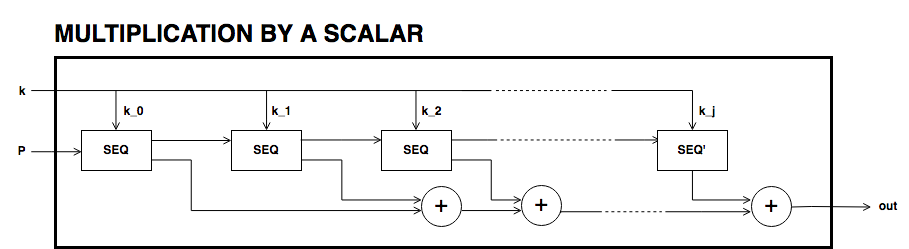
\includegraphics[scale=0.45]{Diag/Mult_by_scalar.png}
	\end{figure}
	
	\item Each \textsc{seq} box takes a point of $E$ of the from $P_i = 2^{248 i} P$ for $i=0,\dots,j-1$ and outputs two points %of $E$,
		$$ 	
			2^{248} \cdot P_i 
			\quad \text{and} \quad
			\sum_{n = 0}^{247} b_n \cdot 2^{n} \cdot P_i. 
		$$
	The first point is the input of the next $(i+1)$-th \textsc{seq} box (note that $ 2^{248} \cdot P_i = P_{i+1}$) whereas the second output is the computation of the $i$-th term in expression (\ref{kP}). The precise circuit is depicted in next two figures \textsc{seq} and \textsc{window}.
	
	\begin{figure}[h]
		\centering
		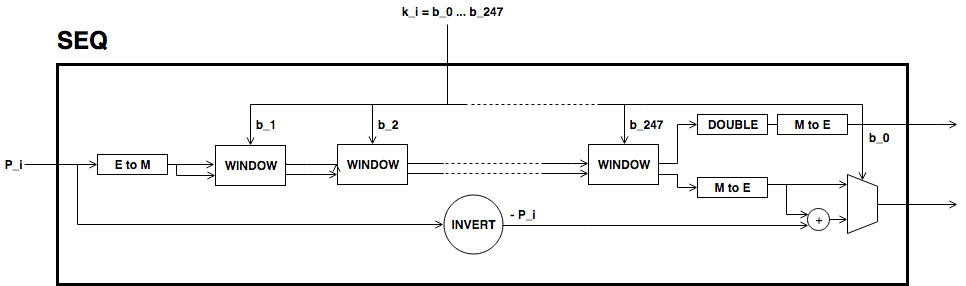
\includegraphics[scale=0.43]{Diag/Mult_by_scalar_SEQ.png}\\
		\vspace{0.5cm}
		
		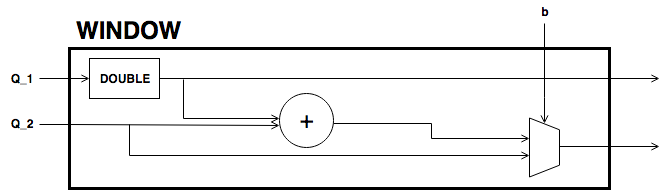
\includegraphics[scale=0.45]{Diag/Mult_by_scalar_SEQ_window.png}
		\vspace{0.3cm}
	\end{figure}

	The idea of the circuit is to first compute some point 		
		$$	Q = P_i + b_1 \cdot (2P_i) + b_2 \cdot (4P_i) 
				+ b_3 \cdot (8P_i) + \dots + b_{247} \cdot (2^{247}P_i), $$
	and output the point
		$$ Q - b_0 \cdot P_i. $$
	This permits the computation of $Q$ using the Montgomery form of Baby-Jubjub and only use twisted Edwards for the second calculation. The reason to change forms is that, in the calculation of the output, we may get a sum with input the point at infinity if $b_0 = 0$. 

	Still, we have to ensure that none of the points being doubled or added when working in $E_M$ is the point at infinity and that we never add the same two points. 

	\begin{itemize}
		
		% None of the points being doubled is the point at infinity.
		\item By assumption, $P\not= O$ and ord$(P)>8$. Hence, by Lagrange theorem {\cite[Corollary 4.12]{lagrange}}, $P$ must have order $r$, $2r$, $4r$ or $8r$. 
		For this reason, none of the points in $E_M$ being doubled or added in the circuit is the point at infinity, because for any integer $m$,  $2^m$ is never a multiple of $r$, even when $2^m$ is larger than $r$, as $r$ is a prime number. Hence, $2^m \cdot P \not= O$ for any $m\in\Z$.		

		% Addition: different points.
		\item Looking closely at the two inputs of the sum, it is easy to realize that they have different parity, one is an even multiple of $P_i$ and the other an odd multiple of $P_i$, so they must be different points. Hence, the sum in $E_M$ is done correctly.
	\end{itemize}
	
	\item The last term of expression (\ref{kP}) is computed in a very similar manner. The difference is that the number of bits composing $k_j$ may be shorter and that there is no need to compute $P_{j+1}$, as there is no other \textsc{seq} box after this one. So, there is only output, the point $k_j \cdot P_j = k_j\cdot 2^{248j} P$. This circuit is named \textsc{seq'}.
	
	\begin{figure}[h]
		\centering
		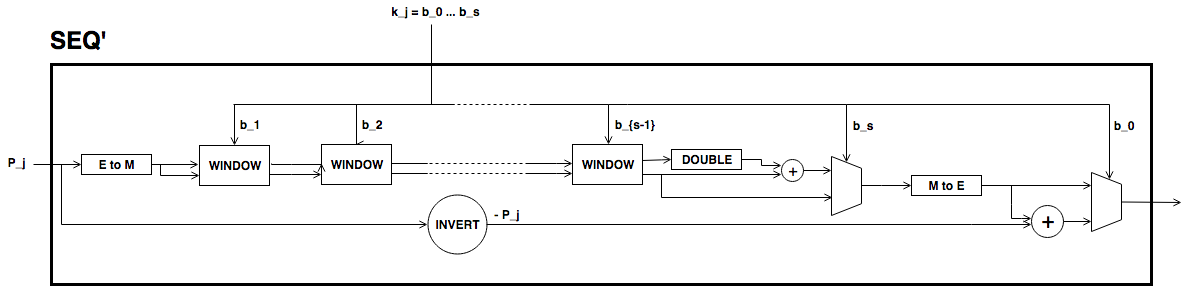
\includegraphics[scale=0.43]{Diag/Mult_by_scalar_SEQ_prime.png}
	\end{figure}
	
\end{enumerate}


\section{Challenges And Security}
	%	If relevant, provide a proof of security in the description.
	As required in the construction of Baby-Jubjub, the curve satisfies SafeCurves criteria. This can be checked following \cite{github-barry}.
	
\section{Implementation}		%	%	If relevant, submit an open source prototype implementation (by including a reference to the repository with the code).

% Others (entry?)
Nonce? of a claim?

Types of entries: claims, etc. D'una part en treiem el lloc on ho guardem i a l'altre etc.		
	Barry WhiteHat:	
	\begin{itemize}
		\item %Description, generation and cryptographic requirements:
		\url{https://github.com/barryWhiteHat/baby_jubjub}
		\item \url{https://github.com/barryWhiteHat/baby_jubjub_ecc} 
	\end{itemize}
	Jordi Baylina: \url{https://github.com/iden3/circomlib/blob/master/src/babyjub.js}
	
\section {Intellectual Property}
	%	We aim to ensure that proposals can be freely implemented. Thus, proposals should disclose the existence of any known patents (awarded or pending) which may restrict free implementation. This may affect the decision process, and a detailed policy is being developed.
%	Creative Commons.

%	\newpage
	\addcontentsline{toc}{section}{References}
	\bibliographystyle{acm}
	\bibliography{lit}
\end{spacing}	
\end{document}
